\documentclass[10pt,journal,compsoc]{IEEEtran}\usepackage[T1]{fontenc}                              % Indicamos la codificacion de las fuentes.
\usepackage[utf8x]{inputenc}                          % Definimos la codificacion.
\usepackage{lmodern}                                  % Para poder usar acentos.
\usepackage[spanish,es-nodecimaldot]{babel}           % Usaremos idioma español y punto decimal.
\usepackage{listings}                                 % Para código
\usepackage[numbered,framed]{matlab-prettifier}       % Para código M
\usepackage{graphicx}
\usepackage{hyperref} 
% para imagenes


% *** CITATION PACKAGES ***
%
\ifCLASSOPTIONcompsoc
  % The IEEE Computer Society needs nocompress option
  % requires cite.sty v4.0 or later (November 2003)
  \usepackage[nocompress]{cite}
\else
  % normal IEEE
  \usepackage{cite}
\fi
% cite.sty was written by Donald Arseneau
% V1.6 and later of IEEEtran pre-defines the format of the cite.sty package
% \cite{} output to follow that of the IEEE. Loading the cite package will
% result in citation numbers being automatically sorted and properly
% "compressed/ranged". e.g., [1], [9], [2], [7], [5], [6] without using
% cite.sty will become [1], [2], [5]--[7], [9] using cite.sty. cite.sty's
% \cite will automatically add leading space, if needed. Use cite.sty's
% noadjust option (cite.sty V3.8 and later) if you want to turn this off
% such as if a citation ever needs to be enclosed in parenthesis.
% cite.sty is already installed on most LaTeX systems. Be sure and use
% version 5.0 (2009-03-20) and later if using hyperref.sty.
% The latest version can be obtained at:
% http://www.ctan.org/pkg/cite
% The documentation is contained in the cite.sty file itself.
%
% Note that some packages require special options to format as the Computer
% Society requires. In particular, Computer Society  papers do not use
% compressed citation ranges as is done in typical IEEE papers
% (e.g., [1]-[4]). Instead, they list every citation separately in order
% (e.g., [1], [2], [3], [4]). To get the latter we need to load the cite
% package with the nocompress option which is supported by cite.sty v4.0
% and later.


% *** GRAPHICS RELATED PACKAGES ***
%
\ifCLASSINFOpdf
  % \usepackage[pdftex]{graphicx}
  % declare the path(s) where your graphic files are
  % \graphicspath{{../pdf/}{../jpeg/}}
  % and their extensions so you won't have to specify these with
  % every instance of \includegraphics
  % \DeclareGraphicsExtensions{.pdf,.jpeg,.png}
\else
  % or other class option (dvipsone, dvipdf, if not using dvips). graphicx
  % will default to the driver specified in the system graphics.cfg if no
  % driver is specified.
  % \usepackage[dvips]{graphicx}
  % declare the path(s) where your graphic files are
  % \graphicspath{{../eps/}}
  % and their extensions so you won't have to specify these with
  % every instance of \includegraphics
  % \DeclareGraphicsExtensions{.eps}
\fi
% graphicx was written by David Carlisle and Sebastian Rahtz. It is
% required if you want graphics, photos, etc. graphicx.sty is already
% installed on most LaTeX systems. The latest version and documentation
% can be obtained at: 
% http://www.ctan.org/pkg/graphicx
% Another good source of documentation is "Using Imported Graphics in
% LaTeX2e" by Keith Reckdahl which can be found at:
% http://www.ctan.org/pkg/epslatex
%
% latex, and pdflatex in dvi mode, support graphics in encapsulated
% postscript (.eps) format. pdflatex in pdf mode supports graphics
% in .pdf, .jpeg, .png and .mps (metapost) formats. Users should ensure
% that all non-photo figures use a vector format (.eps, .pdf, .mps) and
% not a bitmapped formats (.jpeg, .png). The IEEE frowns on bitmapped formats
% which can result in "jaggedy"/blurry rendering of lines and letters as
% well as large increases in file sizes.
%
% You can find documentation about the pdfTeX application at:
% http://www.tug.org/applications/pdftex


% *** MATH PACKAGES ***
%
\usepackage{amsmath}
% A popular package from the American Mathematical Society that provides
% many useful and powerful commands for dealing with mathematics.
%
% Note that the amsmath package sets \interdisplaylinepenalty to 10000
% thus preventing page breaks from occurring within multiline equations. Use:
\interdisplaylinepenalty=2500
% after loading amsmath to restore such page breaks as IEEEtran.cls normally
% does. amsmath.sty is already installed on most LaTeX systems. The latest
% version and documentation can be obtained at:
% http://www.ctan.org/pkg/amsmath


% *** SPECIALIZED LIST PACKAGES ***
\usepackage{algorithmic}
% algorithmic.sty was written by Peter Williams and Rogerio Brito.
% This package provides an algorithmic environment fo describing algorithms.
% You can use the algorithmic environment in-text or within a figure
% environment to provide for a floating algorithm. Do NOT use the algorithm
% floating environment provided by algorithm.sty (by the same authors) or
% algorithm2e.sty (by Christophe Fiorio) as the IEEE does not use dedicated
% algorithm float types and packages that provide these will not provide
% correct IEEE style captions. The latest version and documentation of
% algorithmic.sty can be obtained at:
% http://www.ctan.org/pkg/algorithms
% Also of interest may be the (relatively newer and more customizable)
% algorithmicx.sty package by Szasz Janos:
% http://www.ctan.org/pkg/algorithmicx




% *** ALIGNMENT PACKAGES ***
%
%\usepackage{array}
% Frank Mittelbach's and David Carlisle's array.sty patches and improves
% the standard LaTeX2e array and tabular environments to provide better
% appearance and additional user controls. As the default LaTeX2e table
% generation code is lacking to the point of almost being broken with
% respect to the quality of the end results, all users are strongly
% advised to use an enhanced (at the very least that provided by array.sty)
% set of table tools. array.sty is already installed on most systems. The
% latest version and documentation can be obtained at:
% http://www.ctan.org/pkg/array


%\usepackage{mdwmath}
%\usepackage{mdwtab}
% Also highly recommended is Mark Wooding's extremely powerful MDW tools,
% especially mdwmath.sty and mdwtab.sty which are used to format equations
% and tables, respectively. The MDWtools set is already installed on most
% LaTeX systems. The lastest version and documentation is available at:
% http://www.ctan.org/pkg/mdwtools


% IEEEtran contains the IEEEeqnarray family of commands that can be used to
% generate multiline equations as well as matrices, tables, etc., of high
% quality.


%\usepackage{eqparbox}
% Also of notable interest is Scott Pakin's eqparbox package for creating
% (automatically sized) equal width boxes - aka "natural width parboxes".
% Available at:
% http://www.ctan.org/pkg/eqparbox


% *** SUBFIGURE PACKAGES ***
%\ifCLASSOPTIONcompsoc
%  \usepackage[caption=false,font=footnotesize,labelfont=sf,textfont=sf]{subfig}
%\else
%  \usepackage[caption=false,font=footnotesize]{subfig}
%\fi
% subfig.sty, written by Steven Douglas Cochran, is the modern replacement
% for subfigure.sty, the latter of which is no longer maintained and is
% incompatible with some LaTeX packages including fixltx2e. However,
% subfig.sty requires and automatically loads Axel Sommerfeldt's caption.sty
% which will override IEEEtran.cls' handling of captions and this will result
% in non-IEEE style figure/table captions. To prevent this problem, be sure
% and invoke subfig.sty's "caption=false" package option (available since
% subfig.sty version 1.3, 2005/06/28) as this is will preserve IEEEtran.cls
% handling of captions.
% Note that the Computer Society format requires a sans serif font rather
% than the serif font used in traditional IEEE formatting and thus the need
% to invoke different subfig.sty package options depending on whether
% compsoc mode has been enabled.
%
% The latest version and documentation of subfig.sty can be obtained at:
% http://www.ctan.org/pkg/subfig


% *** FLOAT PACKAGES ***
%
%\usepackage{fixltx2e}
% fixltx2e, the successor to the earlier fix2col.sty, was written by
% Frank Mittelbach and David Carlisle. This package corrects a few problems
% in the LaTeX2e kernel, the most notable of which is that in current
% LaTeX2e releases, the ordering of single and double column floats is not
% guaranteed to be preserved. Thus, an unpatched LaTeX2e can allow a
% single column figure to be placed prior to an earlier double column
% figure.
% Be aware that LaTeX2e kernels dated 2015 and later have fixltx2e.sty's
% corrections already built into the system in which case a warning will
% be issued if an attempt is made to load fixltx2e.sty as it is no longer
% needed.
% The latest version and documentation can be found at:
% http://www.ctan.org/pkg/fixltx2e


%\usepackage{stfloats}
% stfloats.sty was written by Sigitas Tolusis. This package gives LaTeX2e
% the ability to do double column floats at the bottom of the page as well
% as the top. (e.g., "\begin{figure*}[!b]" is not normally possible in
% LaTeX2e). It also provides a command:
%\fnbelowfloat
% to enable the placement of footnotes below bottom floats (the standard
% LaTeX2e kernel puts them above bottom floats). This is an invasive package
% which rewrites many portions of the LaTeX2e float routines. It may not work
% with other packages that modify the LaTeX2e float routines. The latest
% version and documentation can be obtained at:
% http://www.ctan.org/pkg/stfloats
% Do not use the stfloats baselinefloat ability as the IEEE does not allow
% \baselineskip to stretch. Authors submitting work to the IEEE should note
% that the IEEE rarely uses double column equations and that authors should try
% to avoid such use. Do not be tempted to use the cuted.sty or midfloat.sty
% packages (also by Sigitas Tolusis) as the IEEE does not format its papers in
% such ways.
% Do not attempt to use stfloats with fixltx2e as they are incompatible.
% Instead, use Morten Hogholm'a dblfloatfix which combines the features
% of both fixltx2e and stfloats:
%
% \usepackage{dblfloatfix}
% The latest version can be found at:
% http://www.ctan.org/pkg/dblfloatfix


%\ifCLASSOPTIONcaptionsoff
%  \usepackage[nomarkers]{endfloat}
% \let\MYoriglatexcaption\caption
% \renewcommand{\caption}[2][\relax]{\MYoriglatexcaption[#2]{#2}}
%\fi
% endfloat.sty was written by James Darrell McCauley, Jeff Goldberg and 
% Axel Sommerfeldt. This package may be useful when used in conjunction with 
% IEEEtran.cls'  captionsoff option. Some IEEE journals/societies require that
% submissions have lists of figures/tables at the end of the paper and that
% figures/tables without any captions are placed on a page by themselves at
% the end of the document. If needed, the draftcls IEEEtran class option or
% \CLASSINPUTbaselinestretch interface can be used to increase the line
% spacing as well. Be sure and use the nomarkers option of endfloat to
% prevent endfloat from "marking" where the figures would have been placed
% in the text. The two hack lines of code above are a slight modification of
% that suggested by in the endfloat docs (section 8.4.1) to ensure that
% the full captions always appear in the list of figures/tables - even if
% the user used the short optional argument of \caption[]{}.
% IEEE papers do not typically make use of \caption[]'s optional argument,
% so this should not be an issue. A similar trick can be used to disable
% captions of packages such as subfig.sty that lack options to turn off
% the subcaptions:
% For subfig.sty:
% \let\MYorigsubfloat\subfloat
% \renewcommand{\subfloat}[2][\relax]{\MYorigsubfloat[]{#2}}
% However, the above trick will not work if both optional arguments of
% the \subfloat command are used. Furthermore, there needs to be a
% description of each subfigure *somewhere* and endfloat does not add
% subfigure captions to its list of figures. Thus, the best approach is to
% avoid the use of subfigure captions (many IEEE journals avoid them anyway)
% and instead reference/explain all the subfigures within the main caption.
% The latest version of endfloat.sty and its documentation can obtained at:
% http://www.ctan.org/pkg/endfloat
%
% The IEEEtran \ifCLASSOPTIONcaptionsoff conditional can also be used
% later in the document, say, to conditionally put the References on a 
% page by themselves.





% *** PDF, URL AND HYPERLINK PACKAGES ***
%
%\usepackage{url}
% url.sty was written by Donald Arseneau. It provides better support for
% handling and breaking URLs. url.sty is already installed on most LaTeX
% systems. The latest version and documentation can be obtained at:
% http://www.ctan.org/pkg/url
% Basically, \url{my_url_here}.


% NOTE: PDF thumbnail features are not required in IEEE papers
%       and their use requires extra complexity and work.
%\ifCLASSINFOpdf
%  \usepackage[pdftex]{thumbpdf}
%\else
%  \usepackage[dvips]{thumbpdf}
%\fi
% thumbpdf.sty and its companion Perl utility were written by Heiko Oberdiek.
% It allows the user a way to produce PDF documents that contain fancy
% thumbnail images of each of the pages (which tools like acrobat reader can
% utilize). This is possible even when using dvi->ps->pdf workflow if the
% correct thumbpdf driver options are used. thumbpdf.sty incorporates the
% file containing the PDF thumbnail information (filename.tpm is used with
% dvips, filename.tpt is used with pdftex, where filename is the base name of
% your tex document) into the final ps or pdf output document. An external
% utility, the thumbpdf *Perl script* is needed to make these .tpm or .tpt
% thumbnail files from a .ps or .pdf version of the document (which obviously
% does not yet contain pdf thumbnails). Thus, one does a:
% 
% thumbpdf filename.pdf 
%
% to make a filename.tpt, and:
%
% thumbpdf --mode dvips filename.ps
%
% to make a filename.tpm which will then be loaded into the document by
% thumbpdf.sty the NEXT time the document is compiled (by pdflatex or
% latex->dvips->ps2pdf). Users must be careful to regenerate the .tpt and/or
% .tpm files if the main document changes and then to recompile the
% document to incorporate the revised thumbnails to ensure that thumbnails
% match the actual pages. It is easy to forget to do this!
% 
% Unix systems come with a Perl interpreter. However, MS Windows users
% will usually have to install a Perl interpreter so that the thumbpdf
% script can be run. The Ghostscript PS/PDF interpreter is also required.
% See the thumbpdf docs for details. The latest version and documentation
% can be obtained at.
% http://www.ctan.org/pkg/thumbpdf


% NOTE: PDF hyperlink and bookmark features are not required in IEEE
%       papers and their use requires extra complexity and work.
% *** IF USING HYPERREF BE SURE AND CHANGE THE EXAMPLE PDF ***
% *** TITLE/SUBJECT/AUTHOR/KEYWORDS INFO BELOW!!           ***
\newcommand\MYhyperrefoptions{bookmarks=true,bookmarksnumbered=true,
pdfpagemode={UseOutlines},plainpages=false,pdfpagelabels=true,
colorlinks=true,linkcolor={black},citecolor={black},urlcolor={black},
pdftitle={Bare Demo of IEEEtran.cls for Computer Society Journals},%<!CHANGE!
pdfsubject={Typesetting},%<!CHANGE!
pdfauthor={Michael D. Shell},%<!CHANGE!
pdfkeywords={Computer Society, IEEEtran, journal, LaTeX, paper,
             template}}%<^!CHANGE!
%\ifCLASSINFOpdf
%\usepackage[\MYhyperrefoptions,pdftex]{hyperref}
%\else
%\usepackage[\MYhyperrefoptions,breaklinks=true,dvips]{hyperref}
%\usepackage{breakurl}
%\fi
% One significant drawback of using hyperref under DVI output is that the
% LaTeX compiler cannot break URLs across lines or pages as can be done
% under pdfLaTeX's PDF output via the hyperref pdftex driver. This is
% probably the single most important capability distinction between the
% DVI and PDF output. Perhaps surprisingly, all the other PDF features
% (PDF bookmarks, thumbnails, etc.) can be preserved in
% .tex->.dvi->.ps->.pdf workflow if the respective packages/scripts are
% loaded/invoked with the correct driver options (dvips, etc.). 
% As most IEEE papers use URLs sparingly (mainly in the references), this
% may not be as big an issue as with other publications.
%
% That said, Vilar Camara Neto created his breakurl.sty package which
% permits hyperref to easily break URLs even in dvi mode.
% Note that breakurl, unlike most other packages, must be loaded
% AFTER hyperref. The latest version of breakurl and its documentation can
% be obtained at:
% http://www.ctan.org/pkg/breakurl
% breakurl.sty is not for use under pdflatex pdf mode.
%
% The advanced features offer by hyperref.sty are not required for IEEE
% submission, so users should weigh these features against the added
% complexity of use.
% The package options above demonstrate how to enable PDF bookmarks
% (a type of table of contents viewable in Acrobat Reader) as well as
% PDF document information (title, subject, author and keywords) that is
% viewable in Acrobat reader's Document_Properties menu. PDF document
% information is also used extensively to automate the cataloging of PDF
% documents. The above set of options ensures that hyperlinks will not be
% colored in the text and thus will not be visible in the printed page,
% but will be active on "mouse over". USING COLORS OR OTHER HIGHLIGHTING
% OF HYPERLINKS CAN RESULT IN DOCUMENT REJECTION BY THE IEEE, especially if
% these appear on the "printed" page. IF IN DOUBT, ASK THE RELEVANT
% SUBMISSION EDITOR. You may need to add the option hypertexnames=false if
% you used duplicate equation numbers, etc., but this should not be needed
% in normal IEEE work.
% The latest version of hyperref and its documentation can be obtained at:
% http://www.ctan.org/pkg/hyperref





% *** Do not adjust lengths that control margins, column widths, etc. ***
% *** Do not use packages that alter fonts (such as pslatex).         ***
% There should be no need to do such things with IEEEtran.cls V1.6 and later.
% (Unless specifically asked to do so by the journal or conference you plan
% to submit to, of course. )


% correct bad hyphenation here

\hyphenation{op-tical net-works semi-conduc-tor}


\begin{document}
%
% paper title
% Titles are generally capitalized except for words such as a, an, and, as,
% at, but, by, for, in, nor, of, on, or, the, to and up, which are usually
% not capitalized unless they are the first or last word of the title.
% Linebreaks \\ can be used within to get better formatting as desired.
% Do not put math or special symbols in the title.
\title{Proyecto final: DeepFake mediante pix2pix}
%
%
% author names and IEEE memberships
% note positions of commas and nonbreaking spaces ( ~ ) LaTeX will not break
% a structure at a ~ so this keeps an author's name from being broken across
% two lines.
% use \thanks{} to gain access to the first footnote area
% a separate \thanks must be used for each paragraph as LaTeX2e's \thanks
% was not built to handle multiple paragraphs
%
%
%\IEEEcompsocitemizethanks is a special \thanks that produces the bulleted
% lists the Computer Society journals use for "first footnote" author
% affiliations. Use \IEEEcompsocthanksitem which works much like \item
% for each affiliation group. When not in compsoc mode,
% \IEEEcompsocitemizethanks becomes like \thanks and
% \IEEEcompsocthanksitem becomes a line break with idention. This
% facilitates dual compilation, although admittedly the differences in the
% desired content of \author between the different types of papers makes a
% one-size-fits-all approach a daunting prospect. For instance, compsoc 
% journal papers have the author affiliations above the "Manuscript
% received ..."  text while in non-compsoc journals this is reversed. Sigh.

\author{Paul Sebastian~Aguilar Enriquez,
	Carlos Ignacio~Padilla Herrera
	y ~Simón Eduardo~Ramírez Ancona% <-this % stops a space
%\IEEEcompsocitemizethanks{
%  \IEEEcompsocthanksitem Pie 
 % \IEEEcompsocthanksitem Pie
%}% <-this % stops a space
%\thanks{Referencia de pie}
}

% note the % following the last \IEEEmembership and also \thanks - 
% these prevent an unwanted space from occurring between the last author name
% and the end of the author line. i.e., if you had this:
% 
% \author{....lastname \thanks{...} \thanks{...} }
%                     ^------------^------------^----Do not want these spaces!
%
% a space would be appended to the last name and could cause every name on that
% line to be shifted left slightly. This is one of those "LaTeX things". For
% instance, "\textbf{A} \textbf{B}" will typeset as "A B" not "AB". To get
% "AB" then you have to do: "\textbf{A}\textbf{B}"
% \thanks is no different in this regard, so shield the last } of each \thanks
% that ends a line with a % and do not let a space in before the next \thanks.
% Spaces after \IEEEmembership other than the last one are OK (and needed) as
% you are supposed to have spaces between the names. For what it is worth,
% this is a minor point as most people would not even notice if the said evil
% space somehow managed to creep in.



% The paper headers
\markboth{Reconocimiento de patrones, FI-UNAM, 2020-1}%
{Shell \MakeLowercase{\textit{et al.}}: Bare Advanced Demo of IEEEtran.cls for IEEE Computer Society Journals}
% The only time the second header will appear is for the odd numbered pages
% after the title page when using the twoside option.


% for Computer Society papers, we must declare the abstract and index terms
% PRIOR to the title within the \IEEEtitleabstractindextext IEEEtran
% command as these need to go into the title area created by \maketitle.
% As a general rule, do not put math, special symbols or citations
% in the abstract or keywords.

\IEEEtitleabstractindextext{%
\begin{abstract}
Implementar una red neuronal basada en la arquitectura pix2pix que sea capaz de
generar rostros con expresiones faciales distintas a las proporcionadas en el
conjunto de datos de entrenamiento, tomando como referencia la posición de otro
rostro. A esta técnica se le conoce generalmente como \textbf{DeepFake}.

Esta documentación se puede leer más claramente en \href{https://github.com/penserbjorne/face2face}{el repositorio del proyecto}.
\end{abstract}

% Note that keywords are not normally used for peerreview papers.
\begin{IEEEkeywords}
OpenCV, Reconocimiento facial, Segmentación de rostros, pix2pix.
\end{IEEEkeywords}}


% make the title area
\maketitle


% To allow for easy dual compilation without having to reenter the
% abstract/keywords data, the \IEEEtitleabstractindextext text will
% not be used in maketitle, but will appear (i.e., to be "transported")
% here as \IEEEdisplaynontitleabstractindextext when compsoc mode
% is not selected <OR> if conference mode is selected - because compsoc
% conference papers position the abstract like regular (non-compsoc)
% papers do!
\IEEEdisplaynontitleabstractindextext
% \IEEEdisplaynontitleabstractindextext has no effect when using
% compsoc under a non-conference mode.

%
% For peerreview papers, this IEEEtran command inserts a page break and
% creates the second title. It will be ignored for other modes.
\IEEEpeerreviewmaketitle

\section{Objetivo}

El alumno:

\begin{itemize}
  \item Implementara los conocimientos adquiridos durante las materias de Aprendizaje y Reconocimiento de patrones.
\end{itemize}



\section{Introducción}
 
% Here we have the typical use of a "T" for an initial drop letter
% and "HIS" in caps to complete the first word.
\IEEEPARstart{D} eepfake un acrónimo de ``deep learning (aprendizaje profundo)'' y
``fake (falso)'', técnica en la cual se toma a una persona en una imagen
o video existente y se le reemplaza con la imagen de otra persona usando
redes neuronales artificiales.

A menudo se combinan y superponen archivos multimedia existentes en de
origen utilizando técnicas de aprendizaje automático conocidas como
autoencoders y redes de confrontación generativa (Generative Adversarial
Networks, GANs).

\subsubsection{OpenCV}

Es una \textbf{biblioteca libre de visión artificial} originalmente
\textbf{desarrollada por Intel}. Desde que apareció su primera versión
alfa en el mes de enero de 1999, se ha utilizado en infinidad de
aplicaciones. Desde sistemas de seguridad con detección de movimiento,
hasta aplicaciones de control de procesos donde se requiere
reconocimiento de objetos. Esto se debe a que su publicación se da bajo
\textbf{licencia BSD}, que permite que sea usada libremente para
propósitos comerciales y de investigación con las condiciones en ella
expresadas.

Open CV es \textbf{multiplataforma}, existiendo versiones para
GNU/Linux, Mac OS X, Windows y Android. Contiene más de 500 funciones
que abarcan una gran gama de áreas en el proceso de visión, como
reconocimiento de objetos, reconocimiento facial, calibración de
cámaras, visión estérea y visión robótica.

\subsubsection{Detección de rostros con OpenCV}

Desde su versión 3.3, OpenCV cuenta con funciones de \textbf{detección
de rostros basado en aprendizaje profundo}. Estas funciones pertenecen
al módulo de \textbf{redes neuronales profundas (dnn)}.

El módulo de dnn incluye soporte para Caffe, TensorWlof y Torch/PyTorch.
Su principal contribuidor es \textbf{Aleksandr Rybnikov}.

Para utilizar las funciones de detección de rostros del módulo dnn se
requieren los archivos correspondientes con el modelo y los pesos del
mismo.

En el caso de un un modelo con módulos para Caffe, se requieren:

\begin{itemize}
\item
  Archivo \textbf{.prototxt} que define la \textbf{arquitectura del
  modelo}.
\item
  Archivo \textbf{.caffemodel} que contiene los \textbf{pesos} para las
  capas del modelo.
\end{itemize}

El detector facial de aprendizaje profundo de OpenCV se basa en un
\textbf{Single Shot Detector (Detector de disparo único), SSD, con una
red base de ResNet}.

Detección de rostro con el módulo DNN de OpenCV.

\subsubsection{Segmentación de rostros con OpenCV y Dlib} 

\textbf{Dlib es una biblioteca de aprendizaje automático} escrita en
C++. Implementa una amplia gama de algoritmos que se pueden usar en
plataformas de escritorio y móviles.

Dlib permite realizar detección de rostros mediante \textbf{Face
Landmark Localization}. El proceso permite extrapolar un conjunto de
puntos clave a una imagen de un rostro.

Los puntos de referencia (puntos clave) que nos interesan son los que
describen la forma de los atributos de la cara como: ojos, cejas, nariz,
boca y mentón.

Estos puntos dan una idea sobre la estructura de la cara analizada, que
puede ser muy útil para una amplia gama de aplicaciones, que incluyen:
reconocimiento de rostros, animación de rostros, reconocimiento de
emociones, detección de parpadeo y fotografía.

Hay muchos métodos que pueden detectar estos puntos: algunos logran una
precisión y robustez superiores mediante el análisis de un modelo de
cara 3D extraído de una imagen 2D, otros confían en el poder de CNNs
(redes neuronales convolucionales) o RNNs (redes neuronales
recurrentes), y otros más utilizan características simples (pero
rápidas) para estimar la ubicación de los puntos.

El algoritmo \textbf{Face Landmark Detection} ofrecido por Dlib es una
\textbf{implementación del conjunto de árboles de regresión (ERT)}
presentado en 2014 por \textbf{Kazemi y Sullivan}. Esta técnica utiliza
una función simple y rápida de \textbf{diferencias de intensidades de
píxeles} para estimar directamente las posiciones de referencia. Estas
posiciones estimadas se refinan posteriormente con un proceso iterativo
realizado por una \textbf{cascada de regresores}. Los regresores
producen una nueva estimación de la anterior, tratando de reducir el
error de alineación de los puntos estimados en cada iteración. El
algoritmo es increíblemente rápido, de hecho, se necesitan entre 1 y 3
ms (en la plataforma de escritorio) para detectar (alinear) un conjunto
de 68 puntos de referencia en una cara determinada.

Existe un dataset para utilizar adecuadamente el predictor llamado
\textbf{shape\_predictor\_68\_face\_landmarks}, el cual está entrenado
en el conjunto de datos
\textbf{\href{https://ibug.doc.ic.ac.uk/resources/facial-point-annotations/}{ibug
300-W}} de \textbf{C. Sagonas, E. Antonakos, G, Tzimiropoulos, S.
Zafeiriou, M. Pantic.} con 300 caras, y permite indicar mediante un
conjunto de 68 puntos elementos del rostros.

La licencia para este conjunto de datos excluye el uso comercial y
Stefanos Zafeiriou, uno de los creadores del conjunto de datos, pidió
que no puede usarse en un producto comercial.

Para este detector se utilizo una CNN.

\begin{figure}
  \begin{center}
    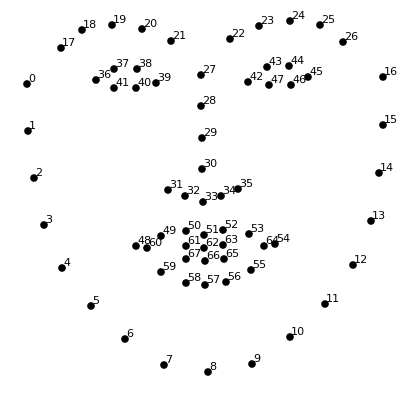
\includegraphics[width=\linewidth]{./imgs/shape_predictor_68_face_landmarks.png}
    \caption{Puntos del predictor llamado shape\_predictor\_68\_face\_landmarks.}
  \end{center}
\end{figure}

\subsubsection{pix2pix (Image-to-Image Translation with Conditional Adversarial Networks)}

\textbf{pix2pix} es el nombre de la arquitectura propuesta en el paper
\textbf{Image-to-Image Translation with Conditional Adversarial
Networks} de Phillip Isola, Jun-Yan Zhu, Tinghui Zhou, Alexei A. Efros
del Berkeley AI Research (BAIR) Laboratory de la UC Berkeley.

El paper es una investigación sobre las redes adversas condicionales
como una solución de propósito general para los problemas de traducción
de imagen a imagen. Estas redes no solo aprenden el mapeo de la imagen
de entrada a la imagen de salida, sino que también aprenden una función
de pérdida para entrenar este mapeo. Esto hace posible aplicar el mismo
enfoque genérico a problemas que tradicionalmente requerirían
formulaciones de pérdidas muy diferentes.

En el paper se demostró que este enfoque es efectivo para sintetizar
fotos a partir de mapas de etiquetas, reconstruir objetos a partir de
mapas de bordes e colorear imágenes, entre otras tareas. Como comunidad,
ya no se diseña a mano las funciones de mapeo, y este trabajo sugiere
que se pueden lograr resultados razonables sin diseñar a mano las
funciones de pérdida.

\textbf{En resumen:}

\begin{itemize}
\item
  Estas redes(cGAN) aprenden el mapeo de la entrada a la salida y una
  función de pérdida para entrenar el mapeo mismo.
\item
  Se vuelve posible aplicar un acercamiento genérico a problemas que
  tradicionalmente requieren diferentes funciones de pérdida.
\end{itemize}

El paper ha tenido tres revisiones (2017, 2018, 2019).

\begin{itemize}
\item \href{https://phillipi.github.io/pix2pix/}{Sitio del proyecto}
\item \href{https://arxiv.org/abs/1611.07004}{Enlace al paper}
\end{itemize}

\subsubsection{Funcionamiento de pix2pix}

\begin{itemize}
\item
  Utiliza una red generativa adversaria condicional (cGAN) para aprender
  el mapeo de la entrada a la salida.
\item
  Utiliza un Generador y un Discriminador.
\item
  El Generador aplica alguna transformación a la entrada para obtener la
  salida.
\item
  El Discriminador compara la imagen de entrada con una desconocida (la
  generada) y trata de de identificar si esta fue producida por el
  generador.
\end{itemize}

\subsubsection{Ejemplo de funcionamiento de pix2pix}

Un ejemplo de imágenes en blanco y negro que deseamos sean coloreadas.
Figura ~\ref{fig:1}.

\begin{figure}[!htb]
  \begin{center}
    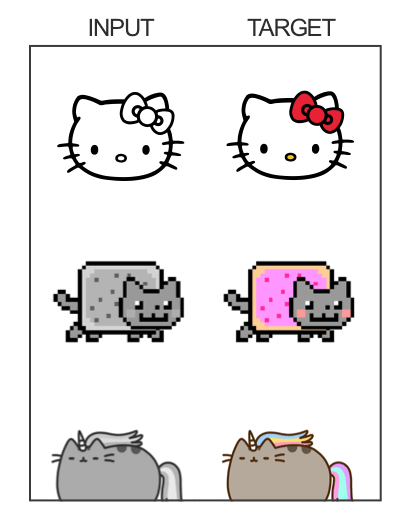
\includegraphics[width=5cm]{./imgs/02_pix2pix_example.png}
    \caption{}
    \label{fig:1}
  \end{center}
\end{figure}

El \textbf{generador} intenta aprender a colorear la imagen. Figura ~\ref{fig:2}

\begin{figure}[!htb]
  \begin{center}
    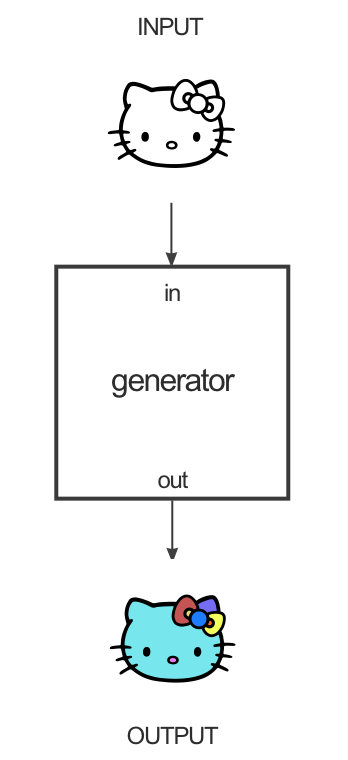
\includegraphics[width=4cm]{./imgs/03_pix2pix_example.png}
    \caption{}
    \label{fig:2}
  \end{center}
\end{figure}

El \textbf{discriminador} analiza la colorización realizada por el
generador e intenta aprender a indicar si la colorización fue correcta o
no.Figura ~\ref{fig:3}

\begin{figure}[!htb]
  \begin{center}
    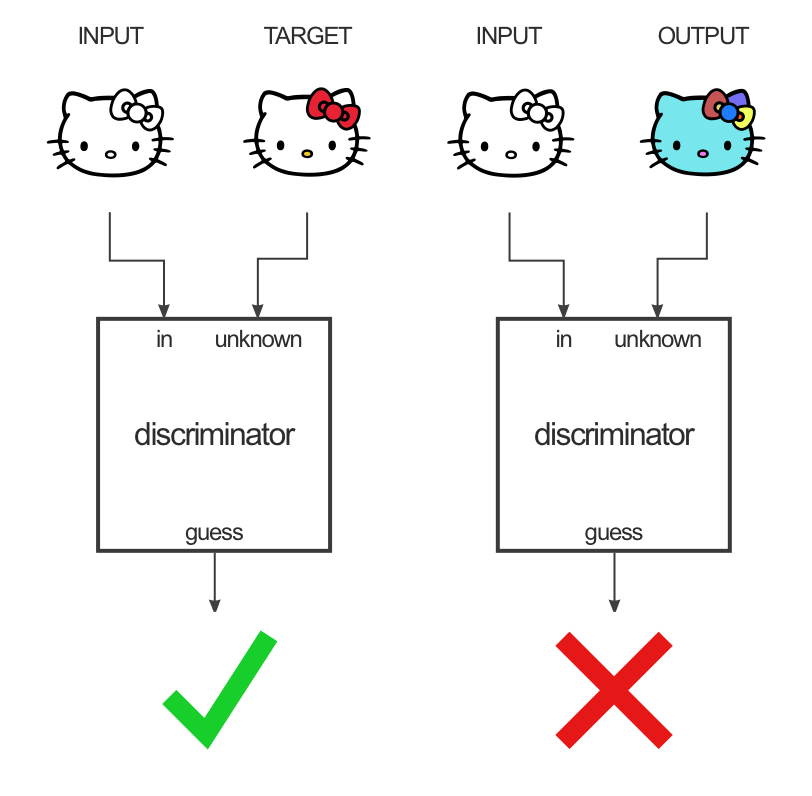
\includegraphics[width=\linewidth]{./imgs/04_pix2pix_example.png}
    \caption{}
    \label{fig:3}
  \end{center}
\end{figure}

El \textbf{generador} utiliza una estructura codificador-decodificador.Figura ~\ref{fig:4}

\begin{figure}[!htb]
  \begin{center}
    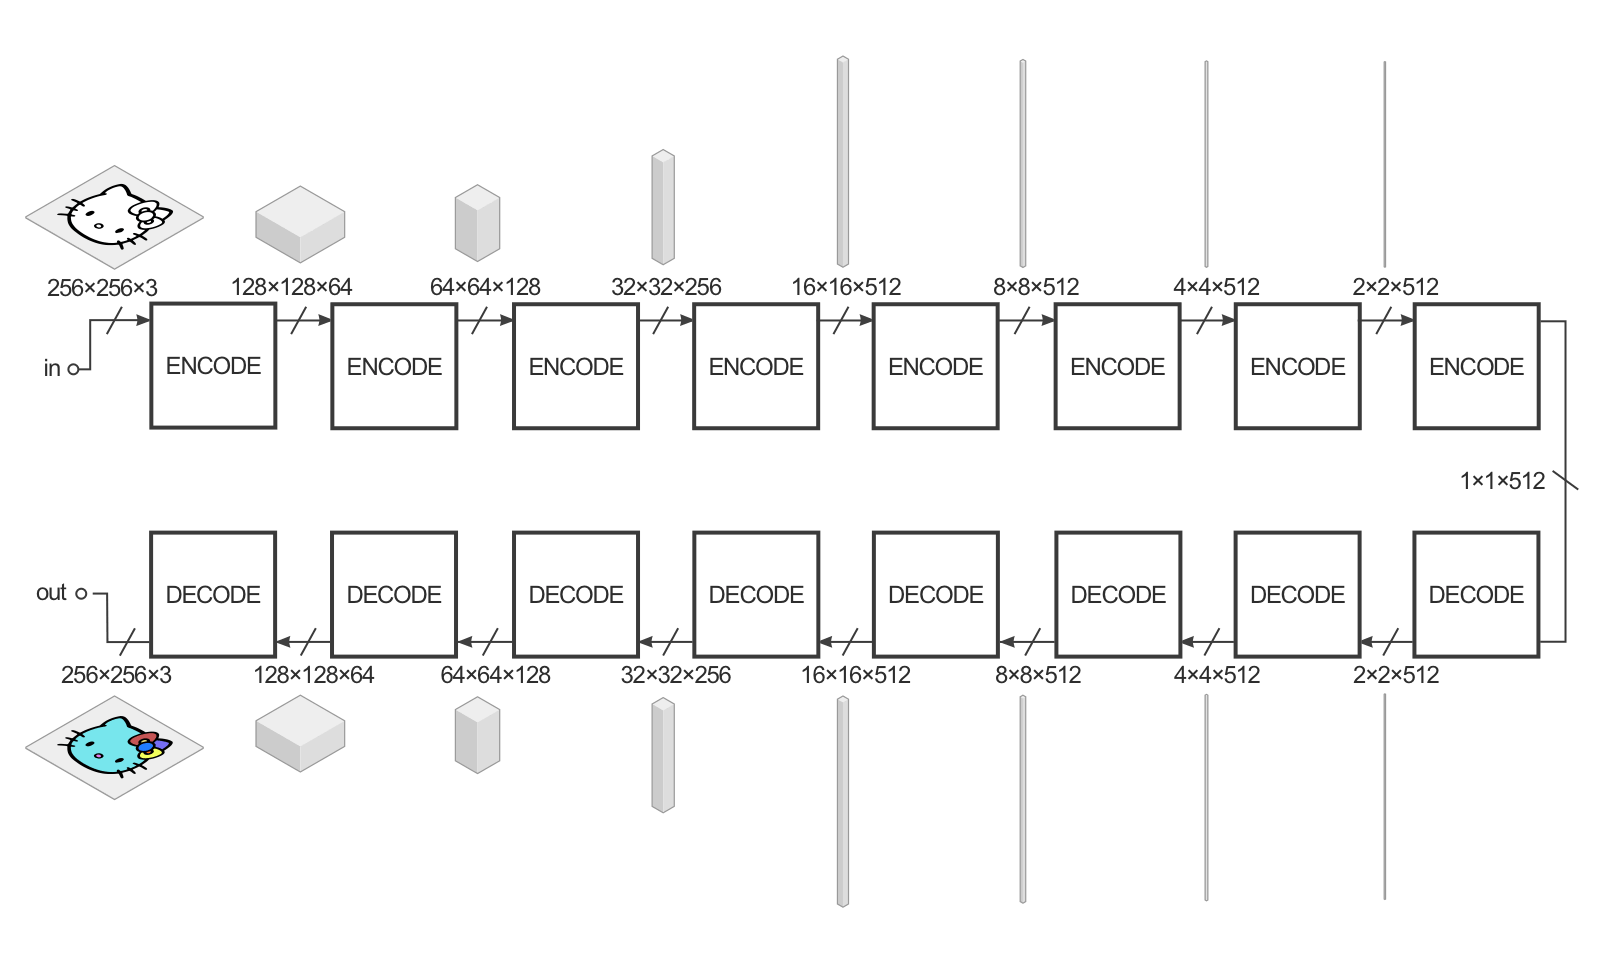
\includegraphics[width=\linewidth]{./imgs/05_pix2pix_example.png}
    \caption{}
    \label{fig:4}
  \end{center}
\end{figure}

\begin{itemize}
\item
  La entrada se intenta reducir con una serie de codificadores
  (convolución + función de activación) en una representación mucho más
  pequeña.
\item
  Al comprimirlo de esta manera, esperamos tener una representación de
  nivel superior de los datos después de la capa de codificación final.
\item
  Las capas de decodificación hacen lo contrario (deconvolución +
  función de activación) e invierten la acción de las capas del
  codificador.
\end{itemize}

Figura ~\ref{fig:5}

\begin{figure}[!htb]
  \begin{center}
    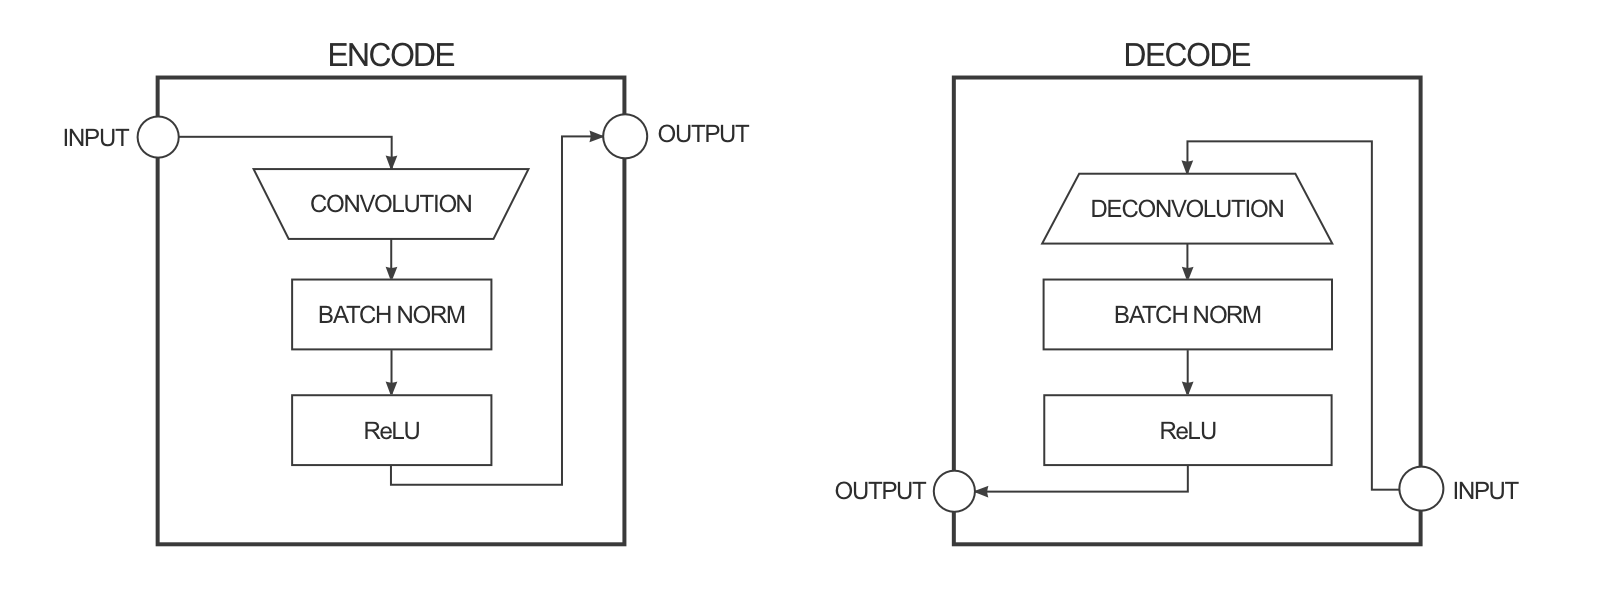
\includegraphics[width=\linewidth]{./imgs/06_pix2pix_example.png}
    \caption{}
    \label{fig:5}
  \end{center}
\end{figure}

Para mejorar el rendimiento de la transformación de imagen a imagen se
utiliza una ``U-Net'' en lugar de un codificador-decodificador. Esto es
lo mismo, pero con ``skip connections (conexiones de omisión)''
conectando directamente las capas del codificador a las capas del
decodificador.

Las conexiones de omisión le dan a la red la opción de omitir la parte
de codificación/decodificación si no tiene un uso para ella. Figura ~\ref{fig:6}

\begin{figure}[!htb]
  \begin{center}
    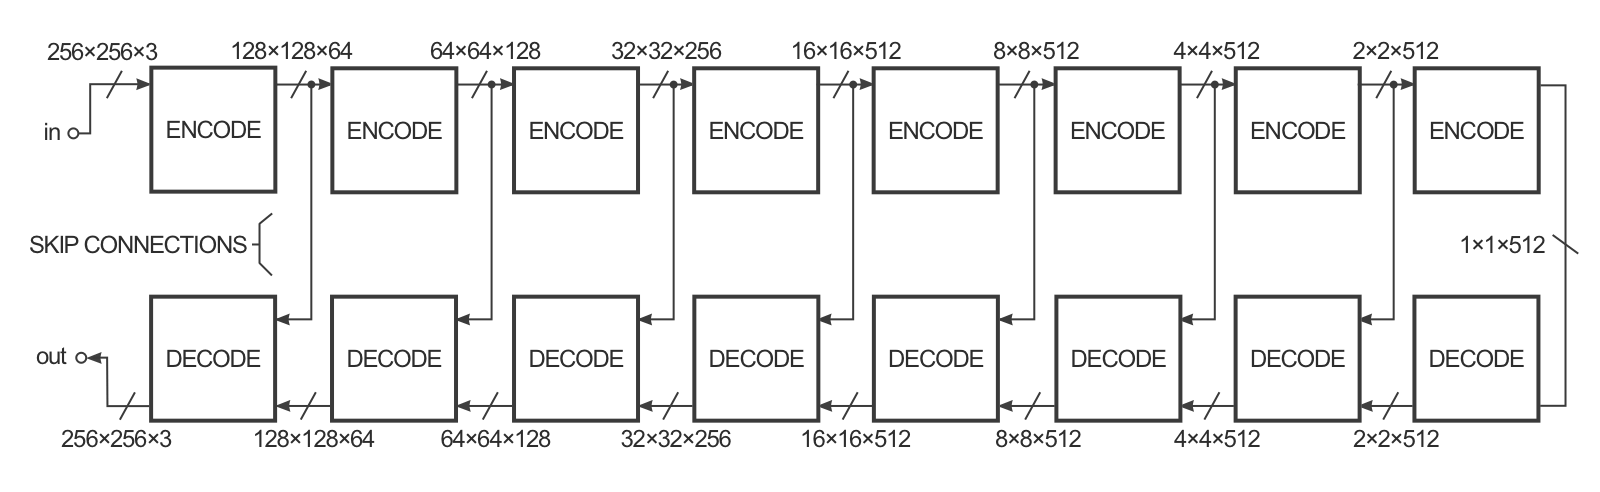
\includegraphics[width=\linewidth]{./imgs/07_pix2pix_example.png}
    \caption{}
    \label{fig:6}
  \end{center}
\end{figure}

El \textbf{discriminador} toma dos imágenes, una imagen de entrada y una
imagen desconocida (que será una imagen objetivo o de salida del
generador), y decide si la segunda imagen fue producida por el generador
o no. La estructura se parece mucho a la sección del codificador del
generador, pero funciona de manera diferente. La arquitectura se llama
\textbf{PatchGAN}. Figura ~\ref{fig:7}

\begin{figure}[!htb]
  \begin{center}
    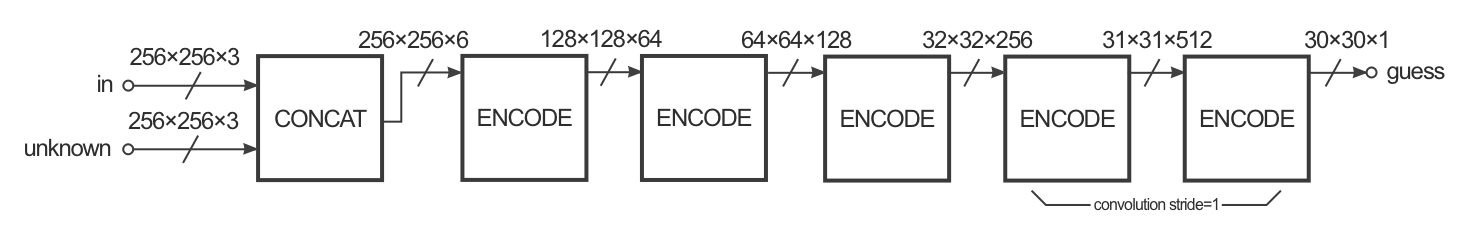
\includegraphics[width=\linewidth]{./imgs/08_pix2pix_example.png}
    \caption{}
    \label{fig:7}
  \end{center}
\end{figure}

\textbf{Para entrenar esta red}, se requiere entrenar al discriminador y
entrenar al generador.

Para entrenar al discriminador, primero el generador genera una imagen
de salida. El discriminador mira el par de entrada/destino y el par de
entrada/salida y genera su conjetura sobre cuán realistas se ven. Los
pesos del discriminador se ajustan en función del error de clasificación
del par de entrada/salida y el par de entrada/destino. Figura ~\ref{fig:8}

\begin{figure}[!htb]
  \begin{center}
    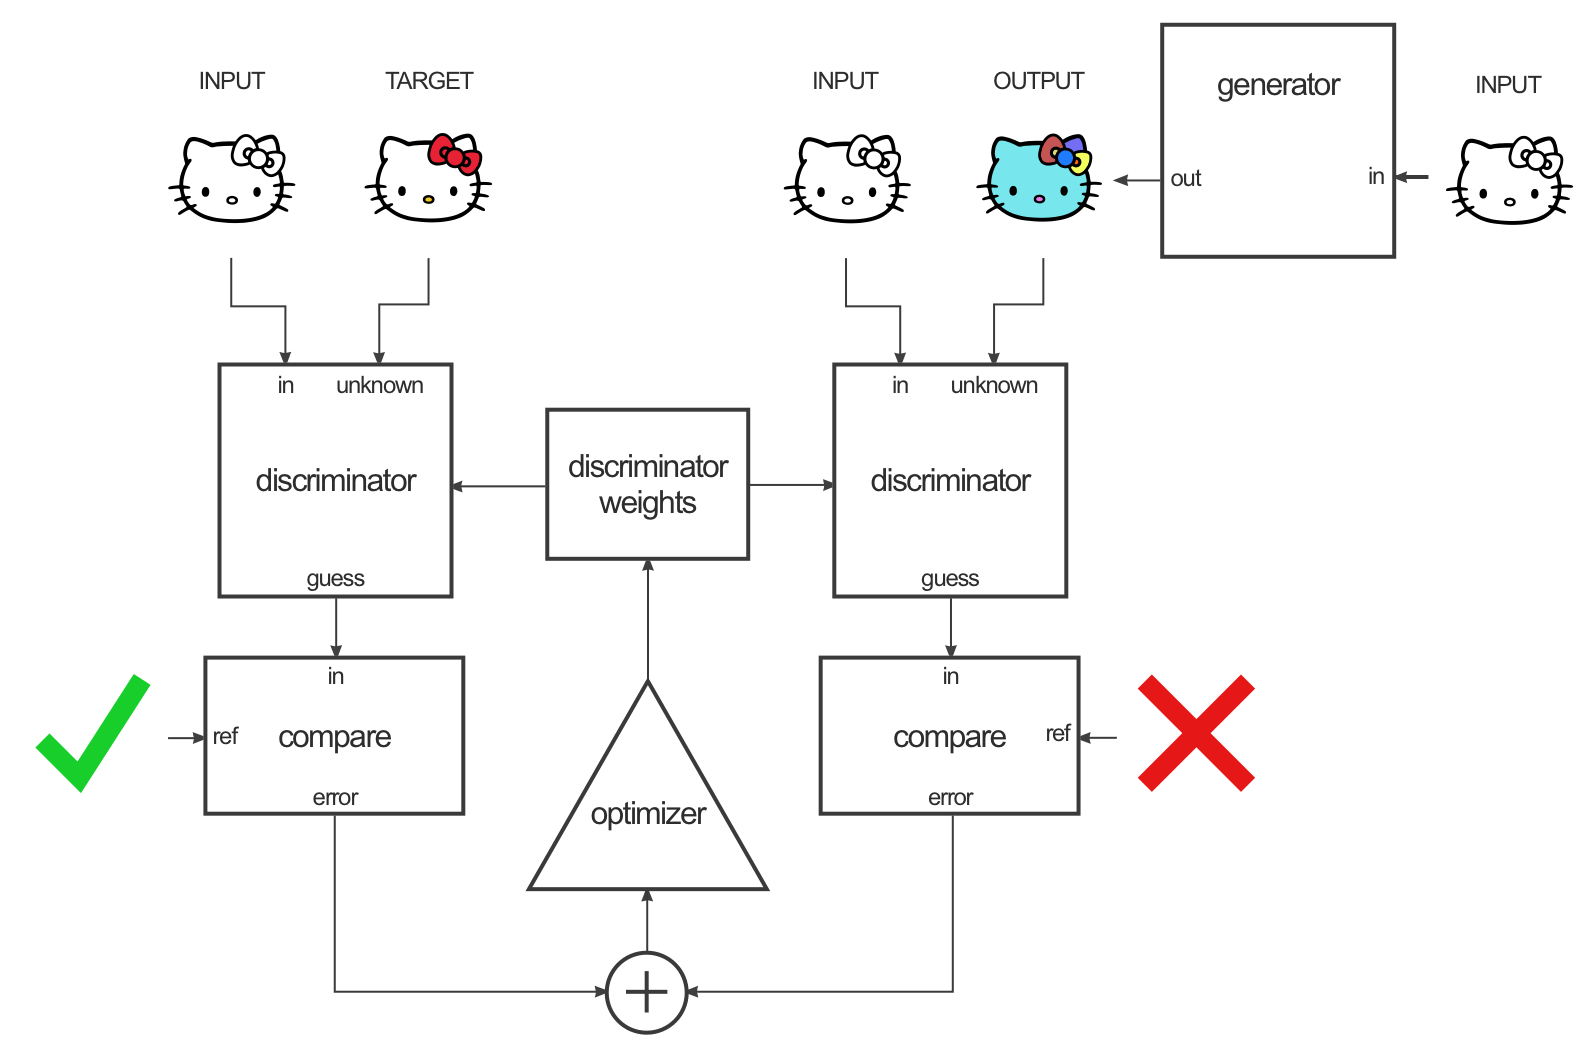
\includegraphics[width=\linewidth]{./imgs/09_pix2pix_example.png}
    \caption{}
    \label{fig:8}
  \end{center}
\end{figure}

Los pesos del generador se ajustan en función de la salida del
discriminador, así como la diferencia entre la imagen de salida y de
destino.

El truco es que cuando entrenas al generador en la salida del
discriminador, en realidad estás calculando los gradientes a través del
discriminador, lo que significa que mientras el discriminador mejora,
estás entrenando al generador para vencer al discriminador.

La teoría es que a medida que el discriminador mejora, también lo hace
el generador. Si el discriminador es bueno en su trabajo y el generador
es capaz de aprender la función de mapeo correcta a través del descenso
de gradiente, debería obtener resultados generados que podrían engañar a
un humano. Figura ~\ref{fig:9}

\begin{figure}[!htb]
  \begin{center}
    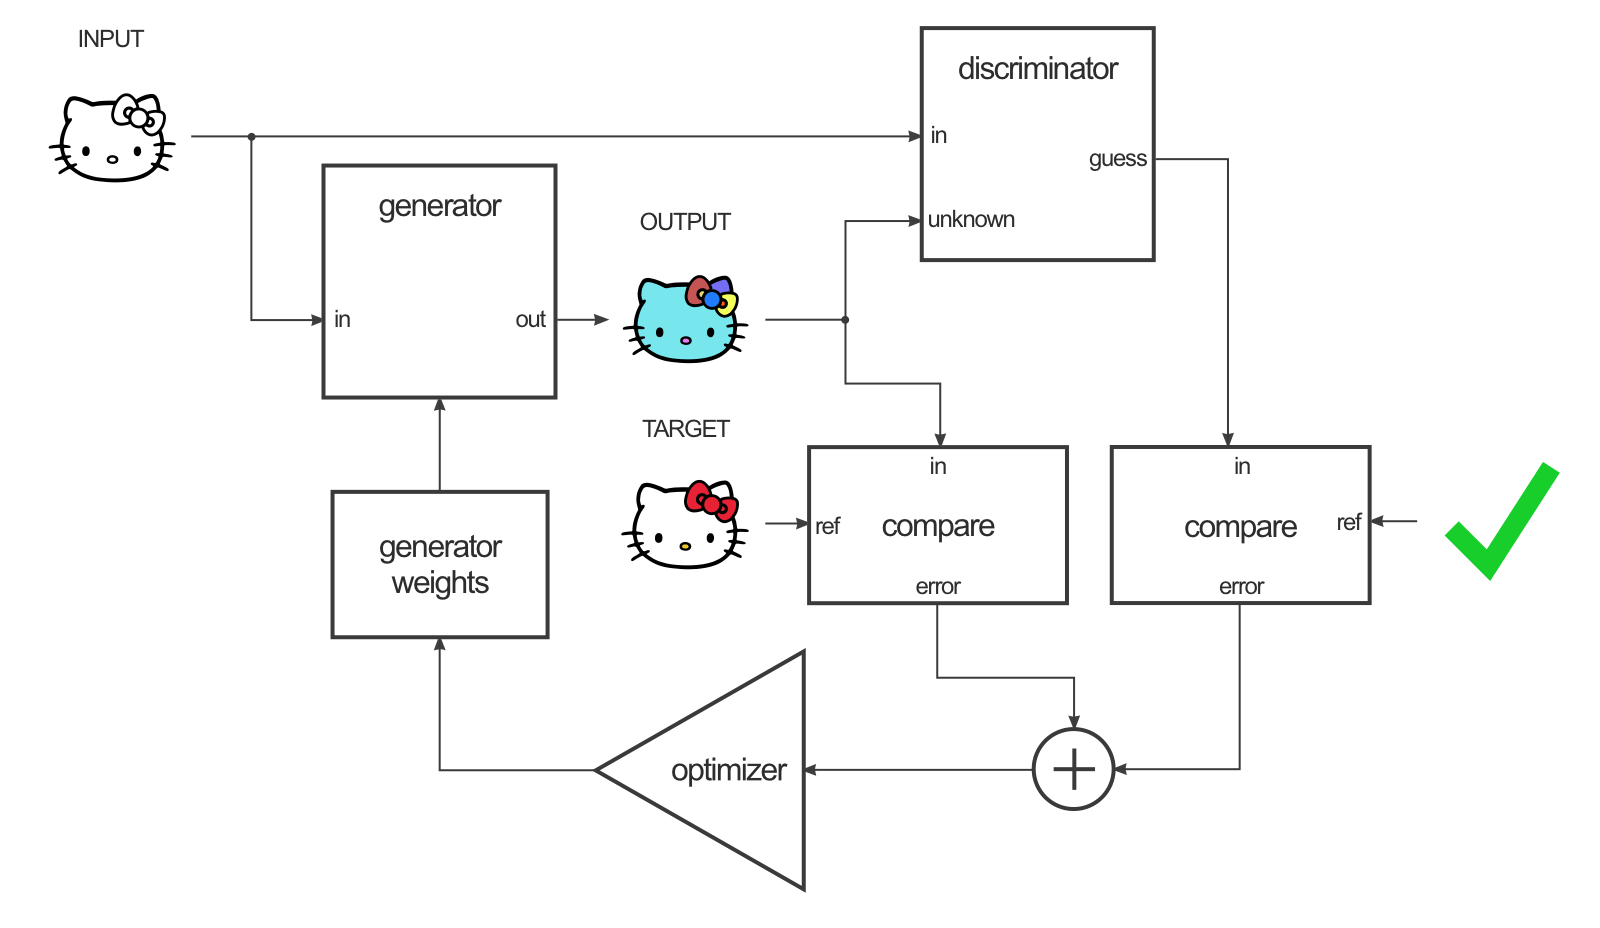
\includegraphics[width=\linewidth]{./imgs/10_pix2pix_example.png}
    \caption{}
    \label{fig:9}
  \end{center}
\end{figure}

Ejemplo de resultados utilizando pix2pix. Figura ~\ref{fig:10}

\begin{figure}[!htb]
  \begin{center}
    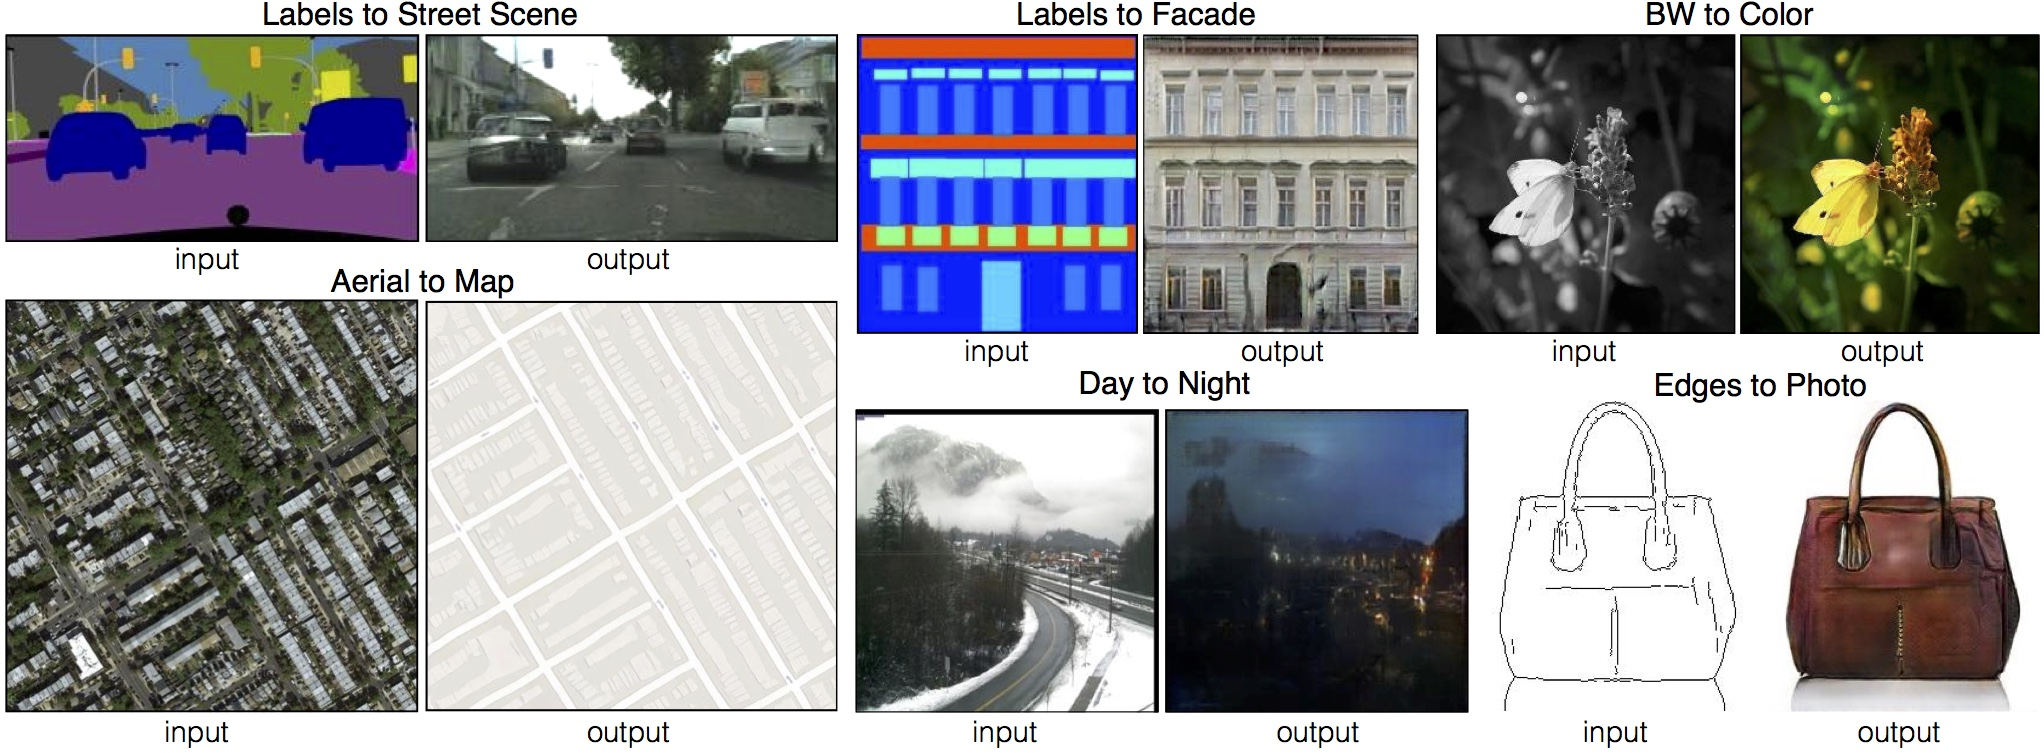
\includegraphics[width=\linewidth]{./imgs/11_pix2pix_example.jpg}
    \caption{}
    \label{fig:10}
  \end{center}
\end{figure}

\hfill

\section{Desarrollo}

El desarrollo del proyecto esta dividido en dos notebooks de
\texttt{Jupyter\ Notebook}.

El primero es para el \textbf{preprocesamiento} y el segundo para la
arquitectura de \textbf{pix2pix}.

\subsection{Implementación}

\paragraph{Preprocesamiento}

El preprocesamiento es para la creación del dataset Se parte de dos
videos de entrada, uno que funcionara para la creación de imágenes de
entrenamiento y otro para la creación de imágenes de prueba. A los
videos se les aplican las siguientes funciones:

\begin{itemize}
\item
  \textbf{Extracción de frames del video:} A través de la biblioteca de
  \texttt{OpenCV} se extraen los frames de este para ser almacenados
  como imágenes. Se puede indicar cada cuantos frames se almacena una
  imagen, esto se puede considerar un parámetro de muestreo. Los frames
  extraidos se almacenan en una carpeta a la cual podemos considerar la
  carpeta de imagenes taggeadas o deseadas a generar.
\item
  \textbf{Detección de rostros en los frames}: Se utiliza un modelo de
  aprendizaje profundo que viene incluido en \texttt{OpenCV}. En esta
  parte se hace la detección del rostro en el frame, y la imagen se
  recorta a un formato de 256x256 con solamente el rostro en ella. La
  imagen se sigue almacenando en la carpeta de de imágenes taggeadas.
\item
  \textbf{Creación de máscaras de rostros a partir de los rostros
  detectados}: Se utiliza la biblioteca \texttt{dlib} junto al algoritmo
  de detección de rostro basado en puntos. Se toman las imágenes
  taggeadas y de cada rostro se hace la detección de sus elementos
  correspondientes: base del rostro, ojos, cejas, nariz y boca. De los
  elementos detectados se genera una máscara con estos y un fondo negro.
  Estas imágenes se almacenan en una carpeta a la cual se considera la
  carpeta de imágenes de entrada.
\end{itemize}

Figura ~\ref{fig:11}, Figura ~\ref{fig:12}, Figura ~\ref{fig:13}

\begin{figure}[!htb]
  \begin{center}
    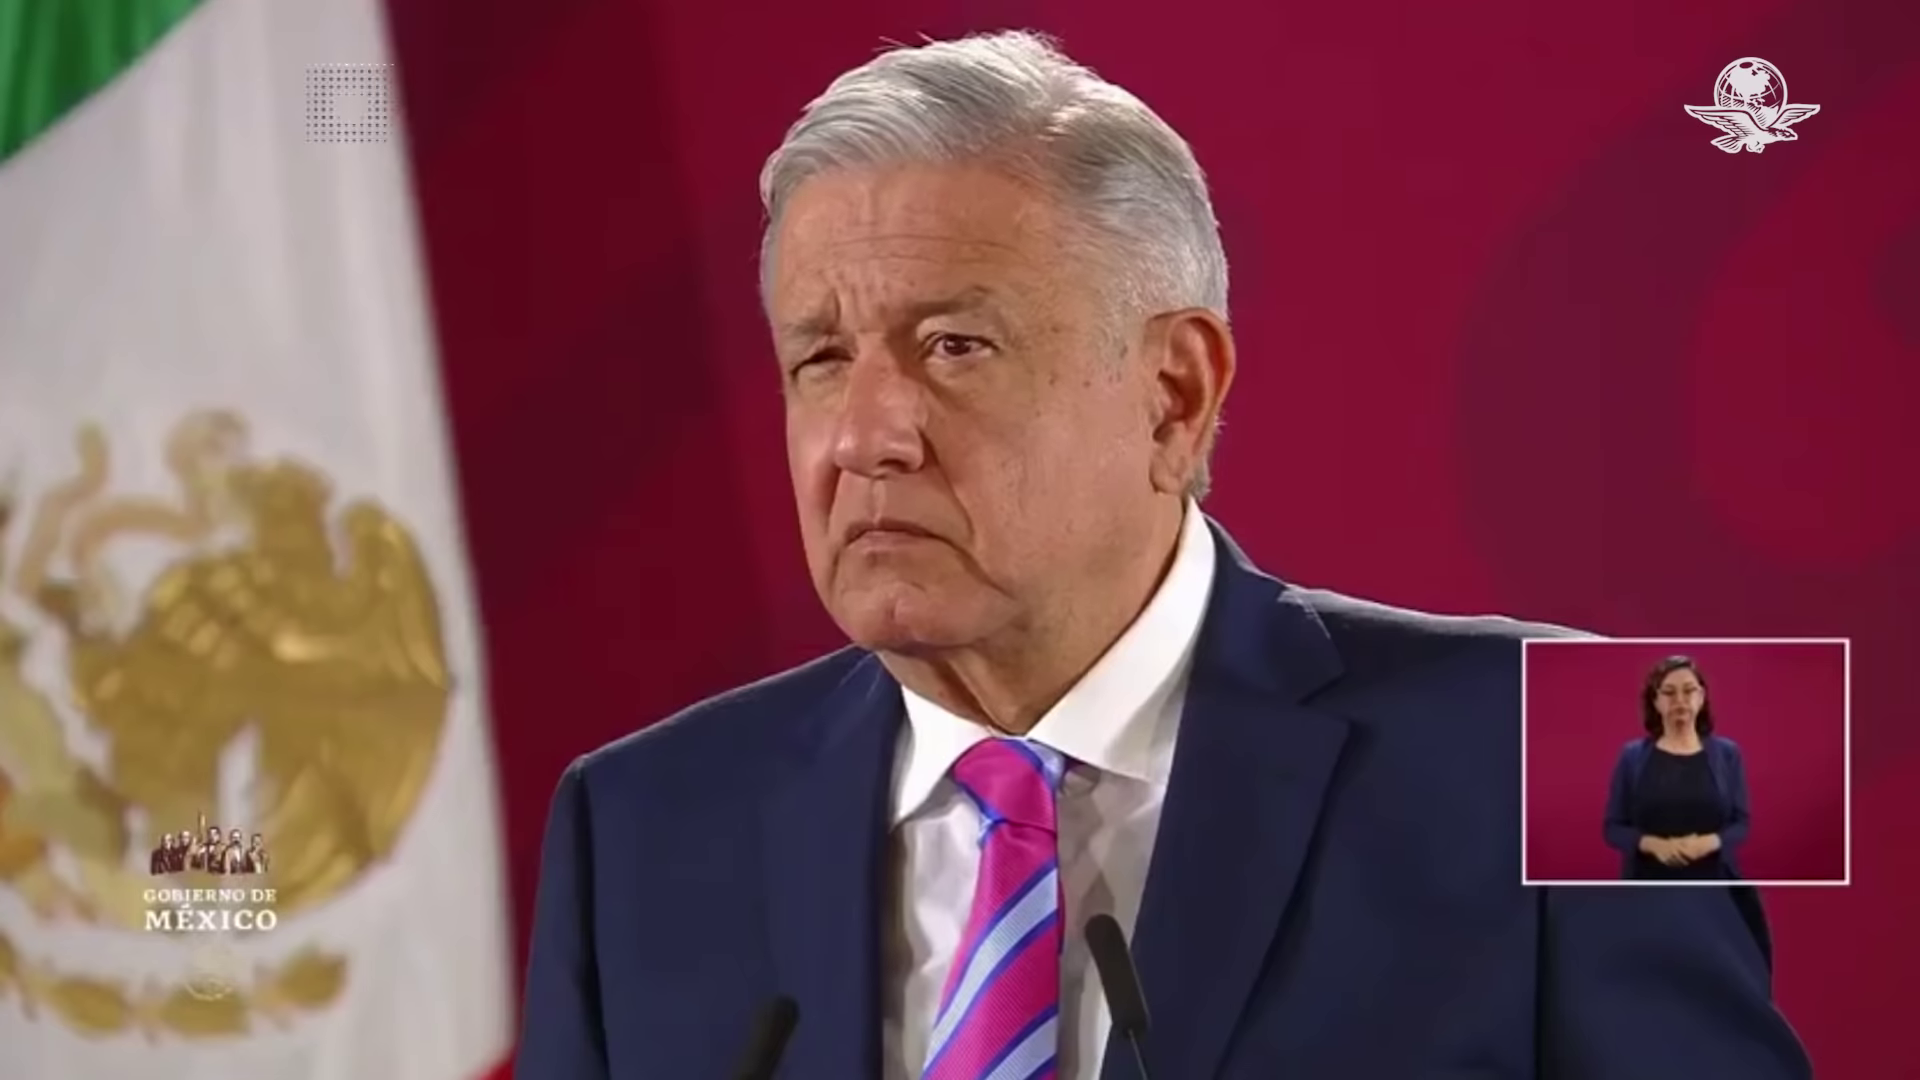
\includegraphics[width=5cm]{./imgs/13_01_frame.png}
    \caption{Frame extraido}
    \label{fig:11}
  \end{center}
\end{figure}

\begin{figure}[!htb]
  \begin{center}
    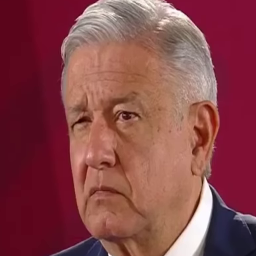
\includegraphics[width=4cm]{./imgs/13_02_rostro.png}
    \caption{Rostro detectado y cortado}
    \label{fig:12}
  \end{center}
\end{figure}

\begin{figure}[!htb]
  \begin{center}
    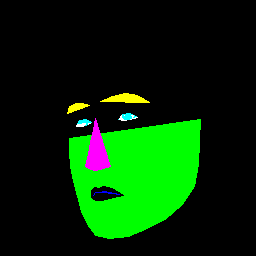
\includegraphics[width=4cm]{./imgs/13_03_mascara.png}
    \caption{Mascara generada}
    \label{fig:13}
  \end{center}
\end{figure}

Figura ~\ref{fig:14}, Figura ~\ref{fig:15}, Figura ~\ref{fig:16}

\begin{figure}[!htb]
  \begin{center}
    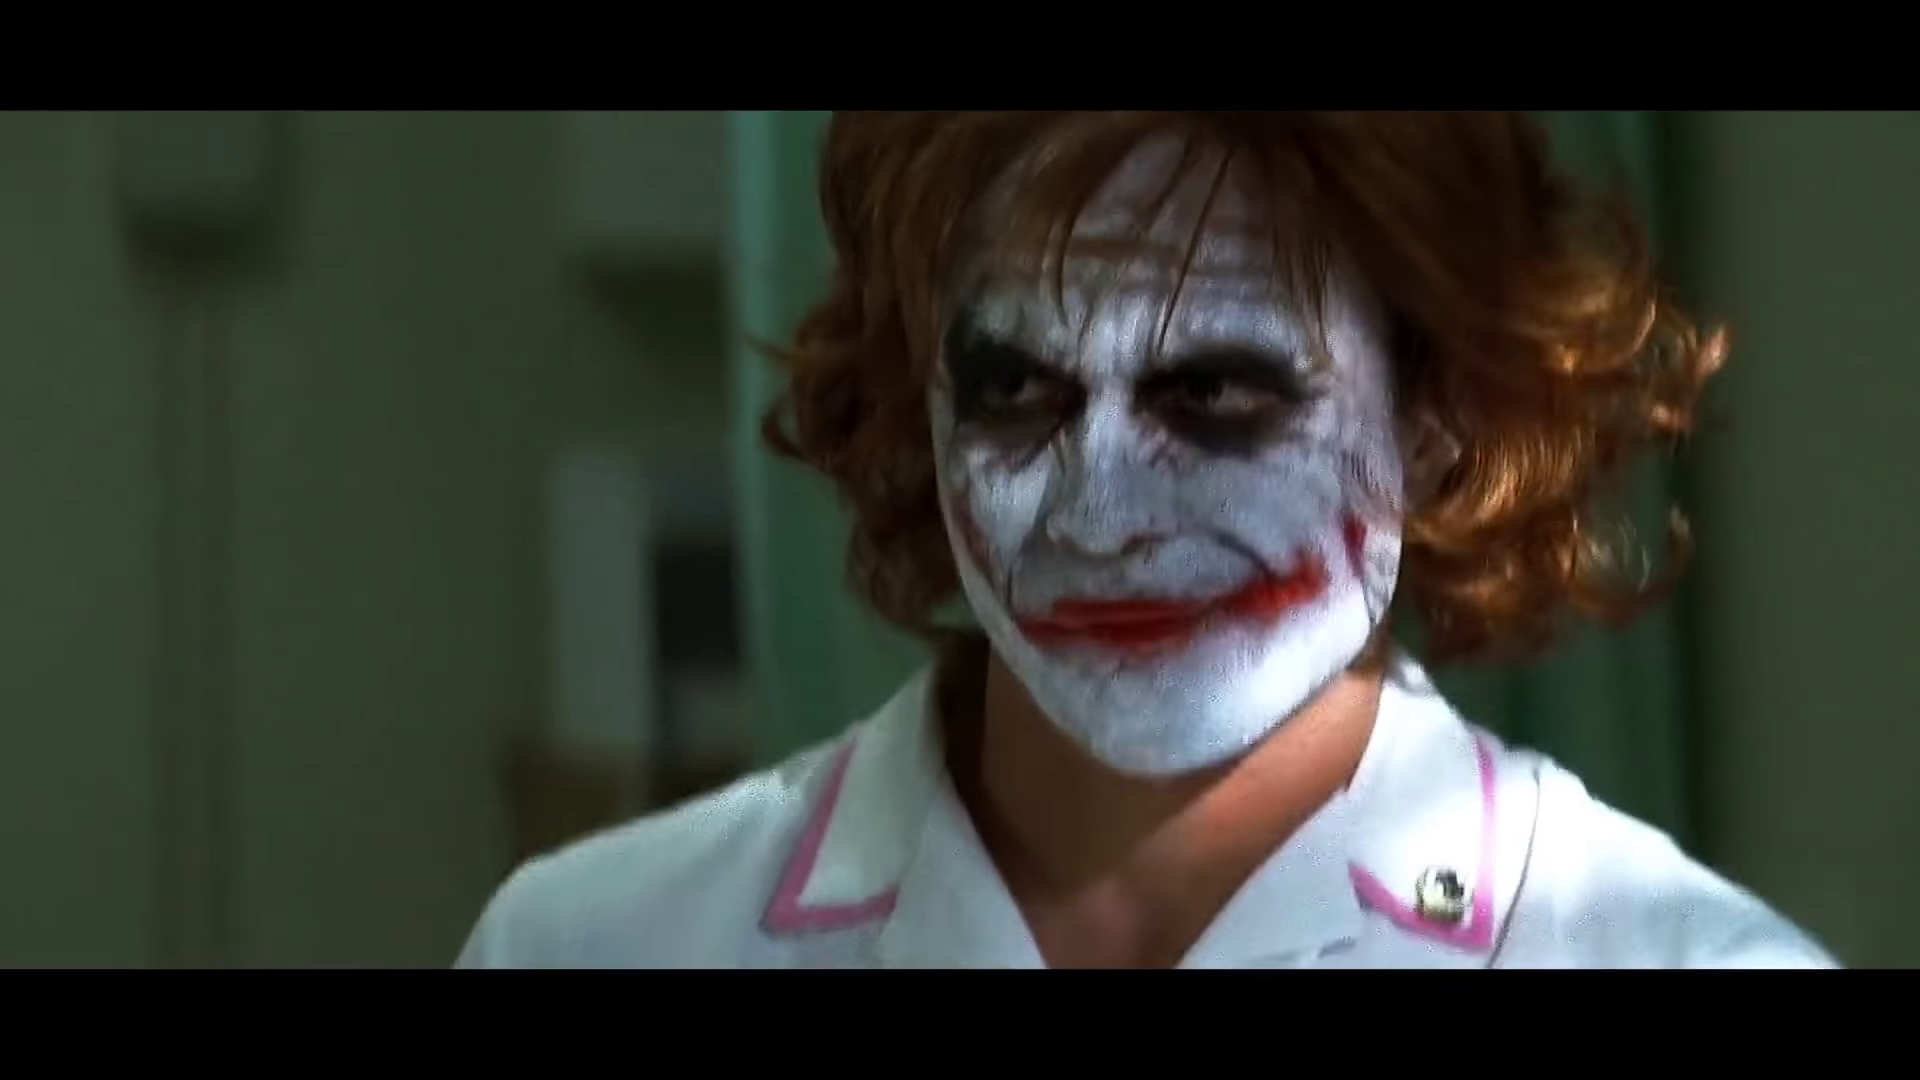
\includegraphics[width=5cm]{./imgs/14_01_frame.png}
    \caption{Frame extraido}
    \label{fig:14}
  \end{center}
\end{figure}

\begin{figure}[!htb]
  \begin{center}
    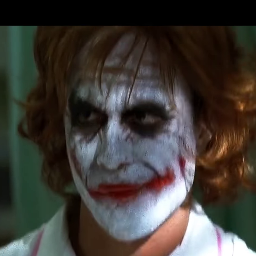
\includegraphics[width=4cm]{./imgs/14_02_rostro.png}
    \caption{Rostro detectado y cortado}
    \label{fig:15}
  \end{center}
\end{figure}

\begin{figure}[!htb]
  \begin{center}
    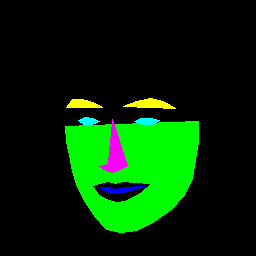
\includegraphics[width=4cm]{./imgs/14_03_mascara.png}
    \caption{Mascara generada}
    \label{fig:16}
  \end{center}
\end{figure}

El preprocesamiento implementado tiene algunos errores, por lo cual hay que
eliminar algunas imágenes a mano ya que no en todos los frames se logra detectar
un rostro, por lo cual no se genera la máscara y hay que eliminarlos para que no
metan ruido a pix2pix.

\paragraph{pix2pix}

La arquitectura implementada es literalmente la propuesta en el paper de
original. Se utilizo \texttt{TensorFlow2} como herramienta de desarrollo
y se configuró para el uso de GPU.

Para la definición del set datos se indican cuatro carpetas. Dos
carpetas corresponden a las imágenes de entrada como máscaras, y dos
corresponden a las imágenes de entrada taggeadas o deseadas a generar
(objetivo). Así como la carpeta de salida.

\begin{lstlisting}[language=Python, basicstyle=\small]
# Definimos carpetas donde se ubican las imagenes
TAGPATHTRAIN = './tagged_train'
INPATHTRAIN = './input_train'
TAGPATHTEST = './tagged_test'
INPATHTEST = './input_test'
OUTPATH = './output'
\end{lstlisting}

Se especifica la cantidad de trabajos para trabajar y el porcentaje que
se utilizara como entrenamiento.

\begin{lstlisting}[language=Python, basicstyle=\small]
# Cantidad de imagenes con las que vamos a trabajar
n = 400
# Porcentaje de nuestro set a ser utilizado como entrenamiento
train_percentage = 0.80
\end{lstlisting}

Como se mencionó, se implementa todo lo indicado en el paper:

\begin{itemize}
\item
  Funciones procesamiento de imágenes

  \begin{itemize}
  \item
    Reescalado
  \item
    Normalización
  \item
    Random jitter
  \end{itemize}
\item
  Carga de imágenes para entrenamiento y prueba
\item
  Bloques básicos para el generador y el discriminador

  \begin{itemize}
  \item
    downsample
  \item
    upsample
  \end{itemize}
\item
  Generador
\item
  Discriminador
\item
  Funciones de costo del generador y del discriminador
\item
  Funciones de medición de rendimiento y carga de imágenes
\item
  Funciones de entrenamiento

  \begin{itemize}
  \item
    Pasos (Incluye el gradiente descendente)
  \item
    Entrenamiento general
  \end{itemize}
\item
  Configuraciones para almacenamiento de checkpoints y optimización
  dentro de TensorFlow
\end{itemize}

Todas estas funciones se utilizan de manera secuencial y se explica el
flujo a continuación:

\begin{itemize}
\item
  Se cargan los set de datos:

  \begin{itemize}
  \item
    Se normalizan a valores de {[}-1, 1{]}.
  \item
    Se indica cual es el set de entrenamiento para que se le apliquen
    operaciones de variación en las imágenes (reescalado, recorte
    aleatorio y espejeo).
  \item
    Se indica cual es el set de prueba para que no se le apliquen
    operaciones de variación en las imágenes.
  \end{itemize}
\item
  Se crea el generador y el discriminador a partir de los bloques de
  upsample y downsample, así como de otras operaciónes.
\item
  Se entrena la red con los siguientes pasos:

  \begin{itemize}
  \item
    Se evalúa la función de costo y se aplica gradiente descendente.
  \item
    Se crea una imagen con el generador.
  \item
    Se compara una imagen con el discriminador.
  \item
    Se hace el ajuste de pesos entre generador y discriminador.
  \end{itemize}
\end{itemize}

La arquitectura de la red queda de la siguiente manera Figura ~\ref{fig:101}, Figura ~\ref{fig:102}:

\begin{figure}[!htb]
  \begin{center}
    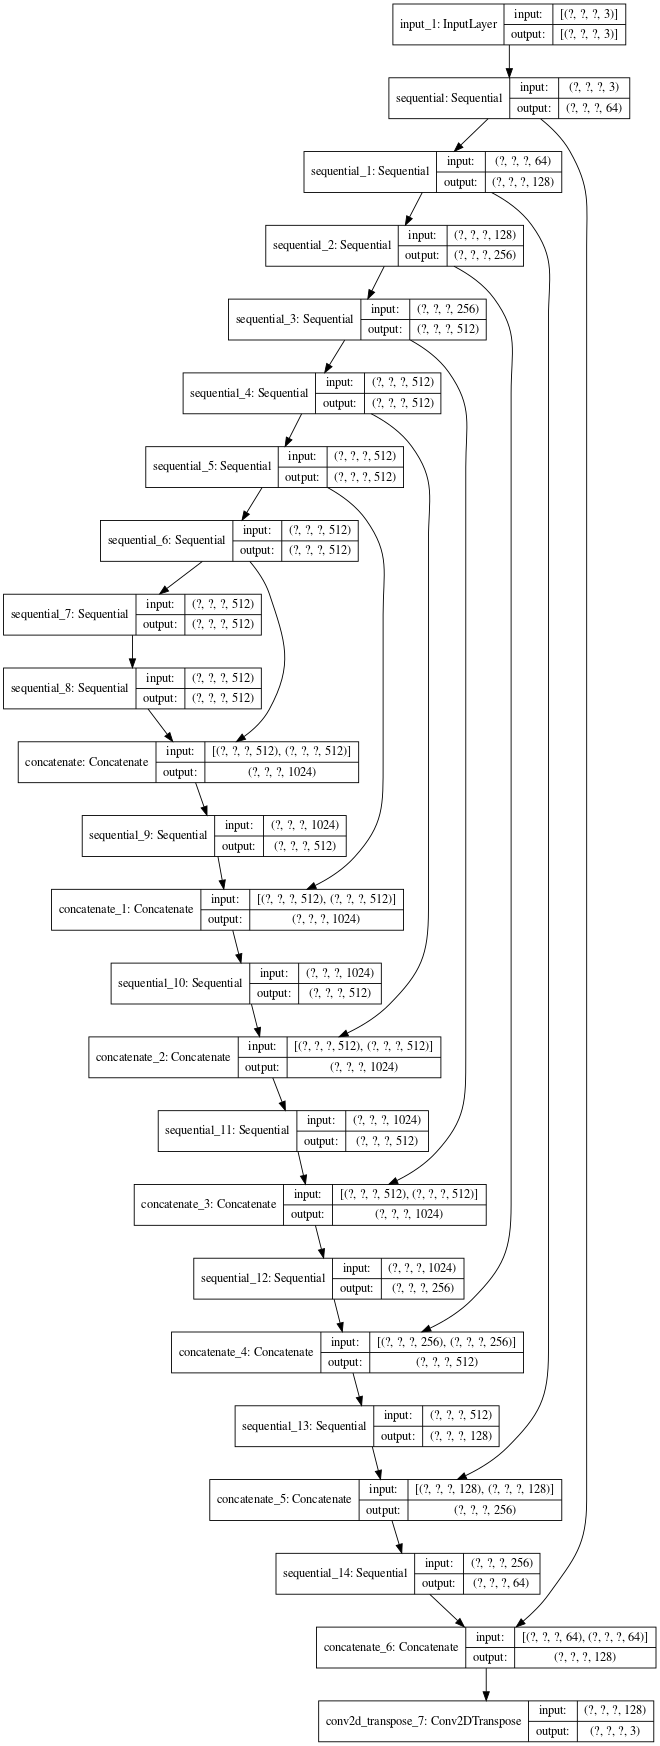
\includegraphics[width=\linewidth]{./imgs/15_generador.png}
    \caption{\textbf{Generador}, basado en una red \textbf{U-Net}.}
    \label{fig:101}
  \end{center}
\end{figure}

\begin{figure}[!htb]
  \begin{center}
    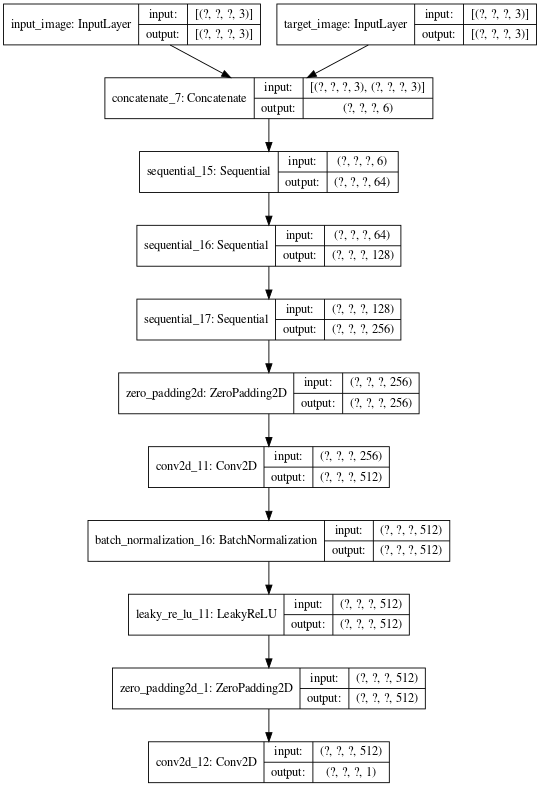
\includegraphics[width=\linewidth]{./imgs/16_discriminador.png}
    \caption{Discriminador, basado en una red \textbf{PatchGAN}.}
    \label{fig:102}
  \end{center}
\end{figure}

\subsection{Requerimientos y Ejecución}

Debido a que \texttt{dlib} solamente funciona hasta
\texttt{python=3.5.6} se tuvieron que crear dos entornos de ejecución.

\paragraph{Preprocesamiento}

\begin{itemize}
\item
  \texttt{Jupyter\ Notebook\ 5.6}
\item
  \texttt{python=3.5.6}
\item
  \texttt{numpy}
\item
  \texttt{opencv}
\item
  \texttt{dlib}
\end{itemize}

\paragraph{pix2pix}

\begin{itemize}
\item
  \texttt{Jupyter\ Notebook\ 6.0.2}
\item
  \texttt{python=3.7.0}
\item
  \texttt{tensorflow-gpu}
\item
  \texttt{matplotlib}
\item
  \texttt{numpy}
\item
  \texttt{pydot}
\item
  \texttt{pillow}
\end{itemize}


\section{Resultados}

Se utilizaron como entrada dos videos. Uno del presidente \textbf{Andrés
Manuel López Obrador en una de ``Las mañaneras''}, y otro de la película
\textbf{El caballero de la noche, de una escena del Joker}.

\begin{itemize}
\item
  \href{https://www.youtube.com/watch?v=BSc32rRlZdM}{AMLO revela cinco
  momentos dificiles de su gobierno}
\item
  \href{https://www.youtube.com/watch?v=YEEsE8snXok}{The Joker \& Harvey
  Dent Two Face / Hospital Scene - The Dark Knight}
\end{itemize}

Se entreno la red con ambos set de datos como prueba y como
entrenamiento.

Las pruebas se realizaron en un equipo:

\begin{itemize}
\item
  Lenovo Legión Y-720
\item
  Sistema Operativo Ubuntu 18.04
\item
  32 GB de RAM
\item
  Tarjeta gráfica GTX 1060 (6 GB de video dedicado)
\item
  Disco de estado solido
\end{itemize}

\subsection{Joker de entrenamiento, AMLO de prueba}

La siguiente prueba se realizo con un set de datos de 400 imágenes, 320
de entrenamiento y 80 de prueba, y un total de 50 epocas. El tiempo que
tardo el entrenamiento fue de 3064.5590 segundos (51.07) minutos.

Figura ~\ref{fig:17}, Figura ~\ref{fig:18}, Figura ~\ref{fig:19}

\begin{figure}[!htb]
  \begin{center}
    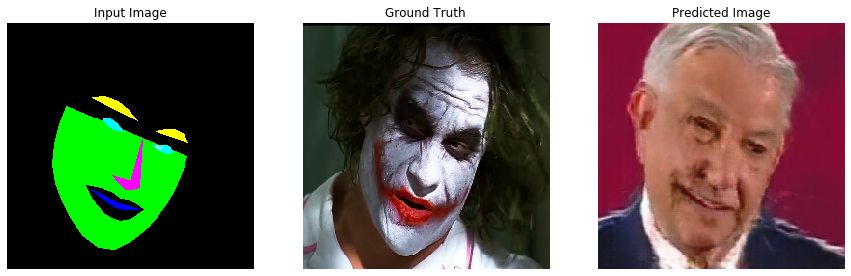
\includegraphics[width=\linewidth]{./imgs/17_01_joker_amlo.png}
    \caption{}
    \label{fig:17}
  \end{center}
\end{figure}

\begin{figure}[!htb]
  \begin{center}
    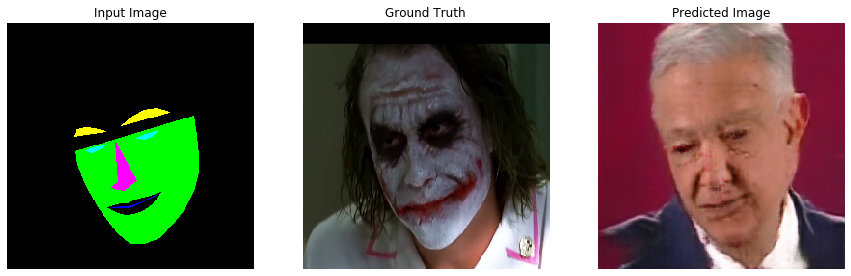
\includegraphics[width=\linewidth]{./imgs/17_02_joker_amlo.png}
        \caption{}
    \label{fig:18}
  \end{center}
\end{figure}

\begin{figure}[!htb]
  \begin{center}
    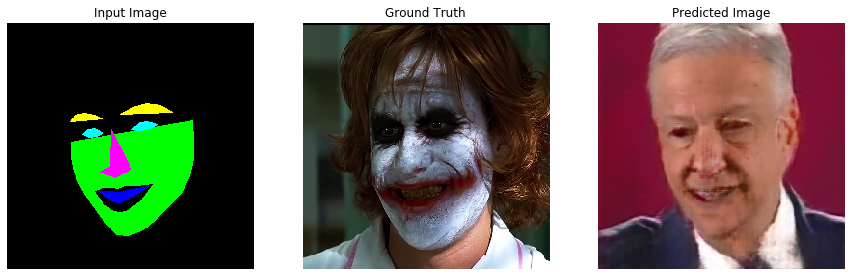
\includegraphics[width=\linewidth]{./imgs/17_03_joker_amlo.png}
        \caption{}
    \label{fig:19}
  \end{center}
\end{figure}

\subsubsection{AMLO de entrenamiento, Joker de prueba}

La siguiente prueba también se realizo con un set de datos de 400
imágenes, 320 de entrenamiento y 80 de prueba, y un total de 50 epocas.
El tiempo que tardo el entrenamiento fue de 3658.7571 segundos (60.97)
minutos.

Figura ~\ref{fig:20}, Figura ~\ref{fig:21}, Figura ~\ref{fig:22}

\begin{figure}[!htb]
  \begin{center}
    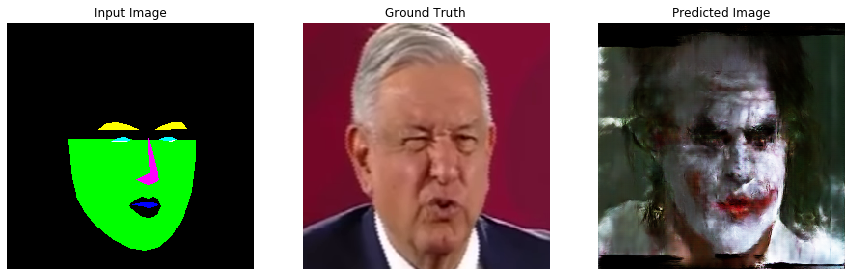
\includegraphics[width=\linewidth]{./imgs/19_01_amlo_joker.png}
        \caption{}
    \label{fig:20}
  \end{center}
\end{figure}

\begin{figure}[!htb]
  \begin{center}
    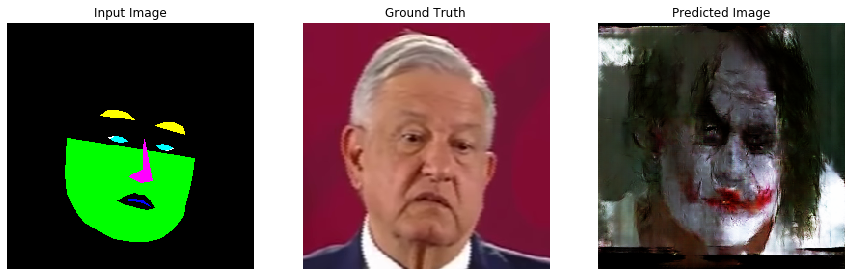
\includegraphics[width=\linewidth]{./imgs/19_02_amlo_joker.png}
        \caption{}
    \label{fig:21}
  \end{center}
\end{figure}

\begin{figure}[!htb]
  \begin{center}
    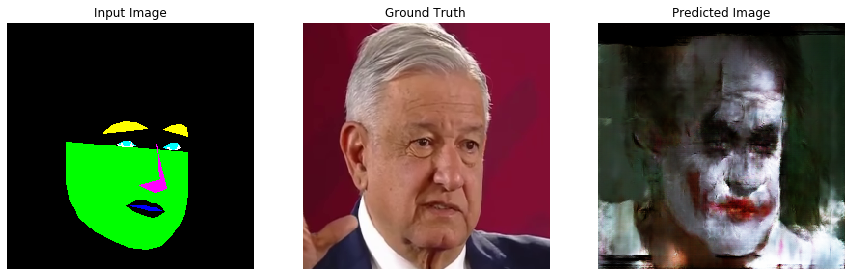
\includegraphics[width=\linewidth]{./imgs/19_03_amlo_joker.png}
        \caption{}
    \label{fig:22}
  \end{center}
\end{figure}

\section{Código fuente}

El código se puede ver en \href{https://github.com/penserbjorne/face2face}{el repositorio del proyecto}.

\section{Conclusiones}
El algortimo de pix2pix es bastante bueno ya que a pesar de tener pocas imagenes en el set de datos de entrenamiento y de pruebas se logró obtener resultados satisfactorios. 

Algo para mejorar seria introducir mas tiempo de procesamiento y un set de imagenes mayor.

% references section

% can use a bibliography generated by BibTeX as a .bbl file
% BibTeX documentation can be easily obtained at:
% http://mirror.ctan.org/biblio/bibtex/contrib/doc/
% The IEEEtran BibTeX style support page is at:
% http://www.michaelshell.org/tex/ieeetran/bibtex/
%\bibliographystyle{IEEEtran}
% argument is your BibTeX string definitions and bibliography database(s)
%\bibliography{IEEEabrv,../bib/paper}
%
% <OR> manually copy in the resultant .bbl file
% set second argument of \begin to the number of references
% (used to reserve space for the reference number labels box)
\section{Referencias}
\begin{itemize}
\item
  \href{https://en.wikipedia.org/wiki/Deepfake}{DeepFake}
\item
  \href{https://es.wikipedia.org/wiki/OpenCV}{OpenCV}
\item
  \href{https://phillipi.github.io/pix2pix/}{Site: Image-to-Image
  Translation with Conditional Adversarial Nets}
\item
  \href{https://affinelayer.com/pix2pix/}{Image-to-Image Translation in
  Tensorflow}
\item
  \href{https://www.pyimagesearch.com/2018/02/26/face-detection-with-opencv-and-deep-learning/\#post_downloads}{Face
  detection with OpenCV and deep learning}
\item
  \href{https://github.com/opencv/opencv/tree/master/samples/dnn/face_detector}{Open
  Source Computer Vision Library}
\item
  \href{https://github.com/arunponnusamy/face-detection-comparison}{Face
  detection using OpenCV and Dlib - A Comparison}
\item
  \href{https://github.com/thegopieffect/computer_vision/tree/master/CAFFE_DNN}{computer\_vision/CAFFE\_DNN}
\item
  \href{https://medium.com/datadriveninvestor/training-alternative-dlib-shape-predictor-models-using-python-d1d8f8bd9f5c}{Training
  alternative Dlib Shape Predictor models using Python}
\item
  \href{https://github.com/davisking/dlib-models}{Trained model files
  for dlib example programs}
\item
  \href{https://github.com/gallardorafael/edge2art}{Edge to Artworks
  translation with Pix2Pix model.}
\item
  \href{https://github.com/RonyBenitez/mimix}{Proyecto DeepFake que
  busca crear en ultima instancia caras falsas usando landmarks del
  controlador o entrada de texto}
\item
  \href{https://www.youtube.com/watch?v=YsrMGcgfETY}{Generando FLORES
  realistas con IA - Pix2Pix \textbar{} IA NOTEBOOK \#5}
\item
  \href{https://www.tensorflow.org/tutorials/generative/pix2pix}{Pix2Pix
  con TensorFlow}
\end{itemize}

% that's all folks
\end{document}
